\section[Reciprocal Lattices]{\hyperlink{toc}{Reciprocal Lattices}}

space in which waves live

not only electron or vibrational waves
-- also waves of light travelling through a crystal

X-rays are used very often to study crystals

\textbf{Recall Reciprocal Lattice in 1D}

\[\sigma x_n = Ae^{i\omega t - i k n a} \]

where:

a = lattice const (direct, in real space)

any system that is periodic in space (a) is also periodic in k space (or reciprocal space) with period $2\pi/a$

Points equivalent to k=0:

\[G_n = \frac{2\pi n}{a}\]

 where n = ... -2, -1, 0, 1, 2, ...
 
 \begin{center}
\begin{tabular}{|c c c c c c c c|} 
 \hline
 \textbf{Space} & ... & n=-2 & n=-1 & n=0 & n=1 & n=2 & ...  \\ [0.5ex] 
 \hline\hline
 $x_n$ =  & ... & -2a & -a & 0 & a & 2a & ... \\ 
 \hline
 $G_n$ =    & ... & -2($\frac{2\pi}{a}$) & -($\frac{2\pi}{a}$) & 0 & ($\frac{2\pi}{a}$)  & 2($\frac{2\pi}{a}$) & ... \\ [1ex] 
 \hline
\end{tabular}
\end{center}


We find a relationship between the spaces:

\begin{tcolorbox}[enhanced,attach boxed title to top center={yshift=-3mm,yshifttext=-1mm},
  colback=blue!5!white,colframe=blue!75!black,colbacktitle=red!80!black,
  title=Reciprocal-Direct Lattice Relationship,fonttitle=\bfseries,
  boxed title style={size=small,colframe=red!50!black} ]
  \begin{equation}
      e^{iG_mx_n} = 1
  \end{equation}
\end{tcolorbox}

\textbf{Reciprocal Lattice now in 3D}

Real:

\[ \textbf{R} = n_1\textbf{a}_1 + n_2\textbf{a}_2 + n_3\textbf{a}_3, \qquad n_i \in  \{0,\pm1, \pm2, \pm3, ...\} \]
 
 Reciprocal:

\[ \textbf{G} = m_1\textbf{b}_1 + m_2\textbf{b}_2 + m_3\textbf{b}_3, \qquad m_i \in  \{0,\pm1, \pm2, \pm3, ...\} \]


Conditions to find vectors of the reciprocal lattice:
\begin{equation}
    e^{\textbf{G}\cdot \textbf{R}} = 1
\end{equation}

construct primitive lattice vectors for the reciprocal lattice \textbf{$b_i$}, using the property that
\begin{equation}
    \textbf{a}_i \cdot \textbf{b}_j = 2 \pi \delta_{ij}
\end{equation}


Ways to determine the reciprocal lattive vectors:
\begin{itemize}
    \item Using a Fourier Transformation of the original lattice (not so intuitive):

\[\rho(x) = \sum_{n} \delta(x-na)\]
\[\mathcal{F}(\rho(x))= \int dx e^{ikx} \rho(x)\]
\[= \sum_n e^{ikan} \]
\[=\frac{2\pi}{a} \sum_m \delta \left(k-\frac{2\pi}{a}m\right) \]


\item Geometric Interpretation: see it as the set of vectors that are normal to the families of lattice planes (infinite set of equidistant parallel lattice planes which as a family contain all of the points of the lattice).

7\item Mathematical Way (minute 1:10 on L8 YT)

Must be equidistant planes and must include ALL points in a crystal.

\pagebreak


\begin{figure}
  \centering
  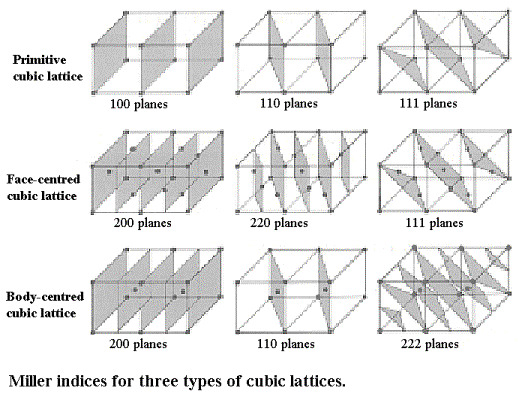
\includegraphics[width=0.6\linewidth]{Images/latticeplanes.jpg}
  \caption{Lattice Planes}
  \label{fig:Lattice Planes}
\end{figure}



\end{itemize}

\textbf{Family of latticce planes:} an infinite set of equidistant parallel lattice planes, which as a family contain all of the points of the lattice.

No extra planes can occur.

\textbf{Index System for Crystal Planes -- Miller Indices}:

\begin{enumerate}
    \item Express the intercepts of the plane with the crystal axes in units of lattice constants a1, a2, a3.
    \item Take the reciprocal of these numbers.
    \item Reduce them to integers of the same ratio: (h,k,l).
\end{enumerate}

\begin{itemize}
    \item round brackets () - reciprocal space
    \item square brackets [] - real space
\end{itemize}

\begin{itemize}
    \item plane parallel to an axis will result in a 0 in the Miller Indices
\end{itemize}

For some experiments it is important to know the distance between the lattice planes

General Distance formula:
\begin{equation}
    d_{hkl} = \frac{n}{\sqrt{\frac{h^2}{a^2}+\frac{k^2}{b^2}+\frac{l^2}{c^2}}}
\end{equation}
Distance for cubic lattice (simpler):
\begin{equation}
    d = \frac{a}{\sqrt{h^2+k^2+l^2}}
\end{equation}

\begin{itemize}
    \item bar over top of miller indice indicates negative number; ex ($11\bar{2}$)
\end{itemize}

\begin{figure}
  \centering
  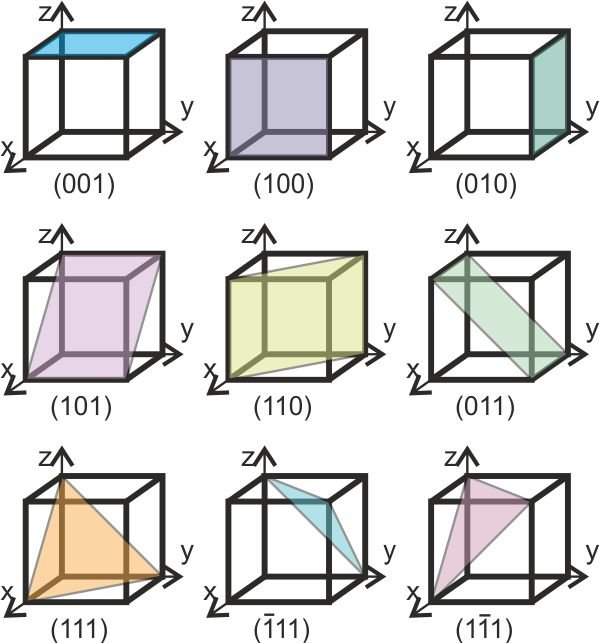
\includegraphics[width=0.6\linewidth]{Images/miller-indices.png}
  \caption{miller indices}
  \label{fig:Miller-Indices}
\end{figure}
